\chapter{Ticketsysteme}
\reiter
\section{Ticketsysteme}
%Quellen: https://www.smartsheet.com/how-use-smartsheet-it-ticketing-system https://de.wikipedia.org/wiki/Issue-Tracking-System 
\subsection{Anmerkung}
Da dieses Dokument eine Event-Management-Software behandelt, in der Tickets, also Eintrittskarten verwaltet und an Promoter vergeben werden, besteht die Gefahr, dass diese Ticketverwaltung mit einem Ticketsystem, also einem Issue-Tracking-System, verwechselt werden kann.  
\subsection{Kartenverwaltungssystem}
Da EMS eine Software zum Managen von Promoter/innen eines Events ist und somit auch die Karten, die ein/e Promoter/in für diese Events zugeteilt bekommt verwaltet werden müssen, musste ein ausführliches Ticketverwaltungssystem erstellt werden.
Für jedes Event können verschieden Kartentypen wie zum Beispiel Early-Bird-, Standart- oder VIP-Karten definiert werden. Sobald ein User einem Event hinzugefügt wird, sieht dieser noch keine Kartentypen. Erst nach einer Transaktion, bei dem ein bestimmter Kartentyp dem User überschrieben wird, sieht er genau die Karten, die er durch eine Transaktion bekommen hat. 
Nachdem ein/e Promoter/in einen bestimmten Kartenstand auf seinem Event-Konto hat, kann er bei Verkauf seinen Kartenstand eintragen. Es wird automatisch das Geld, was er durch diesen Verkauf hat auf der Seite angezeigt. Die Admins können diesen Geld-Soll-Stand sehen und bei einer Übergabe genau überprüfen. 
\subsection{Definition eines Ticketsystems}
Ein Ticketsystem\footcite{issuetracking}, auch Issue-Tracking-System oder Service-Tracking-System, hat die Aufgabe, alle eingehenden Anfrage von internen und externen Stellen zu verwalten. IT-Abteilungen haben ein sehr hohes Volumen von Meldungen, die bewältigt werden müssen. Somit wird ein System benötigt, dass jede einzelne Meldung während des gesamten Lebenszyklus von Eingang bis hin zur Lösung verwaltet.
Es werden verschiedene Dienste bereitgestellt die von einfacher Intake-Software bis hin zu anspruchsvollen Tools, mit denen Probleme ermittelt und verfolgt werden können, reichen.
Ticketsysteme sollen IT-Teams über den Status von Tickets, also gemeldete und formell festgehaltene Probleme, auf dem Laufenden halten und Ihnen helfen, Problemlösungen für diese zu entwickeln. 
Ein Ticket enthält in der Grundform ein technisches Problem, eine Beschreibung des Problems und gegebenenfalls Informationen, die es ermöglichen, dieses Problem zu replizieren.
Ticketsysteme ermöglichen es der IT-Abteilung effizienter zu funktionieren, indem alle Informationen über Probleme, für die die IT-Abteilung Verantwortung trägt, so schnell wie möglich zu lösen, in einem zentralen Datenspeicher in ausreichender Form beschrieben gespeichert werden.
Erfolgreiches Issue-Tracking kann einem Unternehmen helfen Entwicklungskosten von Software zu verringern, da Probleme die frühzeitig behandelt werden einfacher zu beheben sind als jene, die durch fehlende Infrastruktur eines Tracking-Systems erst später behandelt werden können.
\subsection{Funktionsumfang eines Ticketsystems}
\begin{itemize}
	\item \textbf{Self-Service-Portal:} Soll einen One-Stop-Shop darstellen, in dem Kunden und Mitarbeiter ihre Tickets schnell und einfach an die zuständige Abteilung des Unternehmens schicken können. Self-Service-Portale vereinfachen den Kontakt zwischen Kunden bzw. Mitarbeiter und der zuständigen Stelle, indem es genau eine Kontaktstelle gibt. Somit können unnötige Anrufe und E-Mail-Verkehre vermieden werden und optimieren somit den Workflow.
	\item \textbf{Organisationssystem:} Nach Eingang eines Tickets in das System ist der erste Schritt, dieses zu protokollieren. In der Regel werden den Tickets eine prägnante Kategorie, eine Dringlichkeit, eine geschätzte Zeit bis zur Lösung, Fristen und eine Beschreibung, um das Problem, dass das Ticket beschreiben soll, reproduzierbar zu machen, zugewiesen. Die Tickets werden dann in ein Organisationssystem gespeichert und für die Abarbeitung zur Verfügung gestellt.
	\item \textbf{Zuweisen von Tickets:} Um den Workflow des Support-Teams zu optimieren, sollten Tickets im Prinzip des One-Stop-Shops, einen „Eigentümer“, also einen Mitarbeiter, der sich ausschließlich um dieses Ticket kümmert, zugewiesen bekommen. Da eine Abgrenzung zu anderen Tickets besteht muss ein/e Mitarbeiter/in sich nur auf die Tickets konzentrieren, für die er/sie als Eigentümer markiert ist.
	\item \textbf{Sicheres System:} Ticketsysteme sollten sicher sein und somit muss eine hohe Priorität auf die Sicherheit im Auswahlverfahren einer Implementierung gesetzt werden. Informationen, die in einem Ticketsystem gespeichert werden, können interne, systemkritische Probleme beschreiben und müssen damit mit höchster Vertraulichkeit behandelt werden.
	\item \textbf{Live Support:} Ein rund um die Uhr besetzter Helpdesk mit Live-Chat Funktionalität vereinfacht die Meldung von Problemen und fördert somit die Bereitschaft von Kunden und Mitarbeitern aufgetretene Fehler in der Software zu melden und in Kooperation mit dem Support-Team in einer ausreichenden Form zu beschreiben. Der Helpdesk kann bei technischen Problemen, die keine Softwareänderung vermögen, oder auf Seiten des Kunden oder Mitarbeiters entstanden sind mit bereits bekannten Workarounds helfen. Ebenfalls können redundante Tickets vermieden werden, indem das Support-Team kein neues Ticket schreibt, dessen Problem schon erfasst und formell festgehalten wurde.
\end{itemize}
\newpage
Die nachstehenden Funktionen können den Support-Betrieb weiter optimieren
\begin{itemize}
	\item \textbf{Unterstützung für mehrere Kanäle:} Es kann ebenfalls sinnvoll sein, andere Kanäle, wie Telefon, Videochat oder E-Mail, zum Informationsaustausch zur Verfügung zu stellen. Komplexe Probleme können leichter gelöst werden, wenn man in direktem Kontakt mit dem Support-Personal steht. Fragen zu zusätzlichen Themen können beantwortet und Probleme leichter geschildert und mit Hilfe des Personals festgehalten werden. Es bleibt dennoch nur ein formaler Prozess zur Erfassung von Problemen und Formalisierung in ein Ticket bestehen.
	\item \textbf{Dateianhänge:} Kann zur besseren Verständlichkeit des Tickets beitragen. Besonders bei Problemen technischer Natur kann es Hilfreich sein, wenn Informationen wie Memorydumps oder Log-Dateien für den Support zur Verfügung gestellt werden können. Kann zur besseren Verständlichkeit und der Reproduktion von Fehlern eingesetzt werden. Wenn Dateianhänge zugelassen werden sollen, muss ein Dokumentenverwaltungssystem implementiert werden.
	\item \textbf{Mehrsprachige Systeme:} Betrifft hauptsächlich internationale Systeme. Ein Mehrsprachiges Support-System kann dennoch universell sinnvoll sein, da Konversationen in der Muttersprache des Kunden für diesen angenehmer und leichter zu verstehen sind und somit die Bearbeitungszeit der Support-Abteilung verringern können. Internationale Systeme können verschiedensprachige Support-Teams einstellen, die die gewonnen Informationen in einer einheitlichen Sprache, meistens Englisch, im Ticketsystem festhalten. Unternehmen, mit kleineren Budgets können Echtzeitübersetzungsdienste implementieren.
	\item \textbf{Anpassung:} Es ist Sinnvoll, Ticketsysteme mit Orientierung an Plug-and-Play-Prinzipien zu entwickeln, da somit der Funktionsumfang des Systems an die Anforderungen des Projekts angepasst werden kann und eine spätere Erweiterung des Ticketsystems vereinfacht wird.
\end{itemize}  
Die genannten Funktionen stellen allein nicht zwingend sicher, dass das Ticketsystem so effektiv wie möglich funktioniert. Es ist wichtig Kunden, Mitarbeitern und Supportern einen Weg einzurichten, Feedback oder Beschwerden zu äußern und auf dieses zu hören und sich aktiv an der Verbesserung und Anpassung des Ticketsystems zu halten. 
Eine Implementierung eines Berichtssystems, in dem wichtige Metriken und Analysen wie die durchschnittliche Zeit bis zur Problemlösung, Einhaltung von Fristen usw. festgehalten werden kann ebenfalls die Qualität und Effizienz des Supports steigern. 
Community-Foren und regelmäßige Feedback-Umfragen können beim Aufbau und der Pflege von Beziehungen zwischen Support und Kunden helfen und ein Gefühl von Rechenschaftspflicht und Vertrauen erzeugen.
\newpage
%Quelle(n): https://www.datanyze.com/market-share/project-management--217/jira-market-share
\subsection{Marktanalyse}  
Die zunehmenden Anforderungen an Softwareprojekte erzeugen eine steigende Notwendigkeit, fehlerfreie Projekte erfolgreich durchzuführen und die immer weiter steigenden Investitionen in die IT-Branche beschleunigen das Wachstum des weltweiten Issue-Tracking-Markts.
Die mögliche Erhöhung des Return-Of-Investments eines Entwicklers, dass durch die Senkung der Entwicklungskosten bei frühzeitiger Erkennung, Behandlung und Behebung eines Bugs entstehen kann, steigert ebenso die Nachfrage und somit die Wachstumsrate des Markts.
In der folgenden Grafik werden die Marktanteile von den meistverwendeten Ticketsystemen zur Schau gestellt.
Jira sticht hier mit 37.86 Prozent Marktanteil\footcite{marktanteile} als eindeutiger Marktführer heraus. Microsoft Project hat mit 19.09 Prozent einen im Vergleich zu den Nachfolgern einen immer noch sehr hohen Marktanteil.
\begin{figure}[H]
 	\centering
	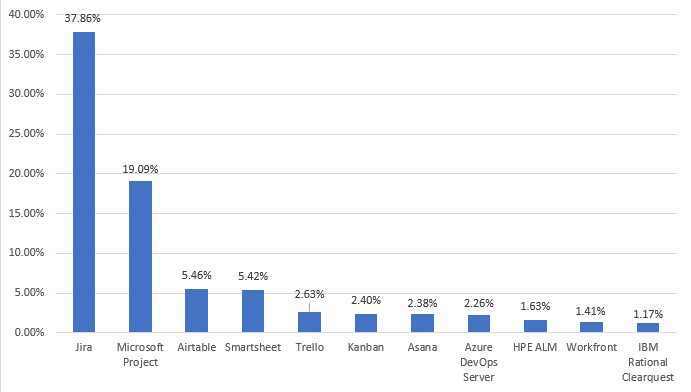
\includegraphics[width=\textwidth]{Marktverteilung_Ticketsysteme.png}
	\caption{Ticketsystem-Marktverteilung}
\end{figure}   
\subsection{Vergleich von Ticketsystemen verschiedener Anbieter}
Es werden die Merkmale der Programme mit Issue-Tracking-Funktionalität
\begin{itemize}
	\item Jira
	\item Microsoft Project
	\item Airtable
	\item Smartsheet
	\item Trello
\end{itemize}
gegenübergestellt.
\newpage  
\subsection{Vergleich}	
%Quellen: https://www.atlassian.com/de/software/jira/features/bug-tracking 
% https://www.atlassian.com/de/software/jira/pricing 
Jira

Jira\footcite{jira} ist ein proprietäres Issue-Tracking-Programm, dass es den Benutzern auch ermöglicht, agiles Projektmanagement zu führen. Jira bietet eine Umfangreiche Implementierung an, die es ermöglicht, Bugs vom Backlog bis zur Behebung zu verfolgen, es können Nachrichten über den aktuellen Status des Fehlers versendet werden, Fehlern können Prioritäten zugewiesen werden, usw…		
Eckdaten:
\begin{itemize}
	\item Kosten:\footcite{jira-pricing} 0\$/Monat Free, 7\$/Benutzer/Monat Standard, 14\$/Benutzer/Monat Premium, Enterprises auf Anfrage
	\item Erstveröffentlichung: 2002
	\item Marktanteil: 37.86\%
\end{itemize}				
Merkmale:
\begin{itemize}
	\item Native Issue-Tracking-Software
	\item Mächtige Implementation des Ticketsystems
\end{itemize}				
%Quellen: https://www.microsoft.com/de-at/microsoft-365/project/compare-microsoft-project-management-software
%https://support.microsoft.com/en-us/office/add-an-issue-to-a-project-in-project-online-3e1a59e5-43b3-4281-9cfb-503c646f49b9 			
Microsoft Project

Microsoft Project\footcite{microsoft-project} ist eine Projektmanagementsoftware, die über eine sehr leichte Implementierung eines Ticketsystems verfügt. Man kann lediglich Issues in einem Project erstellen und wieder löschen.
Eckdaten:
\begin{itemize}
	\item Kosten:\footcite{microsoft-project-pricing} 8.40€/Monat Project Plan 1, 25.30€/Monat Project Plan 3, 46.40€/Monat Project Plan 5
	\item Erstveröffentlichung: 1984
	\item Marktanteil: 19.09\%
\end{itemize}
Merkmale:
\begin{itemize}
	\item Schwache Implementierung des Ticketsystems
\end{itemize}				
%Quellen: https://support.airtable.com/hc/en-us/articles/115003131627-Use-case-bug-issue-tracking-in-Airtable 
%https://airtable.com/templates/product-design-and-ux/expOzMycWirMsUOTL/bug-and-issue-tracker 
%https://airtable.com/pricing 
Airtable

Airtable\footcite{airtable} ist ein Cloud-basierter Kollaborationsdienst der mittels vom Entwickler bereitgestellten Bug Tracker Templates eine Funktionserweiterung als Issue-Tracking-System erhält. Issues können auf einem Kanban board oder auf einem Grid angezeigt werden. Screenshots und Gifs können dem Ticket hinzugefügt werden. Verfügt über mächtige Filteroptionen.	
Eckdaten:
\begin{itemize}
	\item Kosten:\footcite{airtable-pricing} Free, 10\$/Monat Plus, 20\$/Monat Pro, Auf Anfrage Enterprise Package
	\item Erstveröffentlichung: 2012 
	\item Marktanteil: 5.46\%
\end{itemize}
\newpage		
Merkmale:
\begin{itemize}
	\item Screenshot- und Gif-attachment der Tickets
	\item Mächtige Filteroptionen
	\item Cloud-basiert
\end{itemize}
%Quellen: https://www.smartsheet.com/how-use-smartsheet-it-ticketing-system
% https://de.smartsheet.com/pricing 
Smartsheet
			
Smartsheet\footcite{smartsheet} ist eine über Software-as-a-Service laufende Projektmanagement Software und hat ein eingebautes Ticketsystem namens Help Desk Ticket Tracker \& Form. Es optimiert die Ticketverwaltung, indem es interne und externe Tickets organisiert und stellt einen Helpdesk zur Verfügung. 
Eckdaten:
\begin{itemize}
	\item Kosten:\footcite{smartsheet-pricing} 13€/Monat Einzelbenutzer, 22€/Monat Business, Enterprise auf Anfrage
	\item Erstveröffentlichung: 2006
	\item Marktanteil: 5.42\%
\end{itemize}		
Merkmale:
\begin{itemize}
	\item Software-as-a-Service
	\item Native Implementation eines Ticketsystems.
	\item Stellt einen Helpdesk zur Verfügung.
\end{itemize}
%Quellen: https://blog.trello.com/how-to-transform-trello-into-a-powerful-bug-tracker-with-the-marker-power-up
% https://trello.com/de/pricing 				
Trello

Trello\footcite{trello} ist ein Aufgaben-Verwaltungs-Onlinedienst der mittels Marker-Plugin mit einem Issue-Tracking-System erweitert werden kann. Trello versucht im Markt herauszustechen, indem Issue-Tracking um vielfaches vereinfacht wird. Es können eigene Strukturen und Ticketeigenschaften definiert werden. 
Eckdaten:
\begin{itemize}
	\item Kosten:\footcite{trello-pricing} 0\$ Free, 10\$/Monat Business Class, Auf Anfrage Enterprise Package.
	\item Erstveröffentlichung: 2011
	\item Marktanteil: 2.63\%
\end{itemize}		
Merkmale:
\begin{itemize}
	\item Sehr schnelles Set-Up
	\item Sehr Simpel
	\item Eigene Definierung von Ticketeigenschaften und Strukturen
\end{itemize}
\newpage
\subsection{Vergleich zwischen Vivifyscrum und Jira als Issue-Tracking-System}
Im Rahmen der Projektentwicklung musste das Projektmanagement-tool Vivifyscrum als Issue-Tracking-System verwendet werden. Eigentlich war geplant Jira als Projektmanagementsoftware und Issue-Tracking-Tool zu verwendet. In diesem Vergleich werden Vivifyscrum und Jira hinsichtlich Issue-Tracking-Funktionalitäten auf Basis früherer Erfahrungen gegenübergestellt. 

Vivifyscrum
Die Issue-Tracking-Funktionalitäten in Vivifyscrum sind sehr begrenzt. Es gibt keine eigene Implementation für Issues, sondern nur die Möglichkeit, Objekte, die User-Stories sein können, in Bugs oder Ideas umzuändern.

Jira hat dagegen eine sehr mächtige Implementierung eines Issue-Tracking-Systems. Es können Issues erstellt werden, User Stories zu Issues abgeändert werden, Bugs können priorisiert werden und über den kompletten Lebenszyklus des Bugs verfolgt und auf Wunsch kann bei einer Statusänderung des Bugs eine Nachricht verschickt werden. Es ist auch möglich nach vielen verschiedenen Kriterien zu filtern.  